%! Author = Gian Flütsch
%! Date = 21. Jun 2022
%! Project = IncResp Zusammenfassung

\section{Incident Response Prozess}

\subsection{ISO/IEC 27035-1}
\begin{center}
    \vspace{-8pt}
    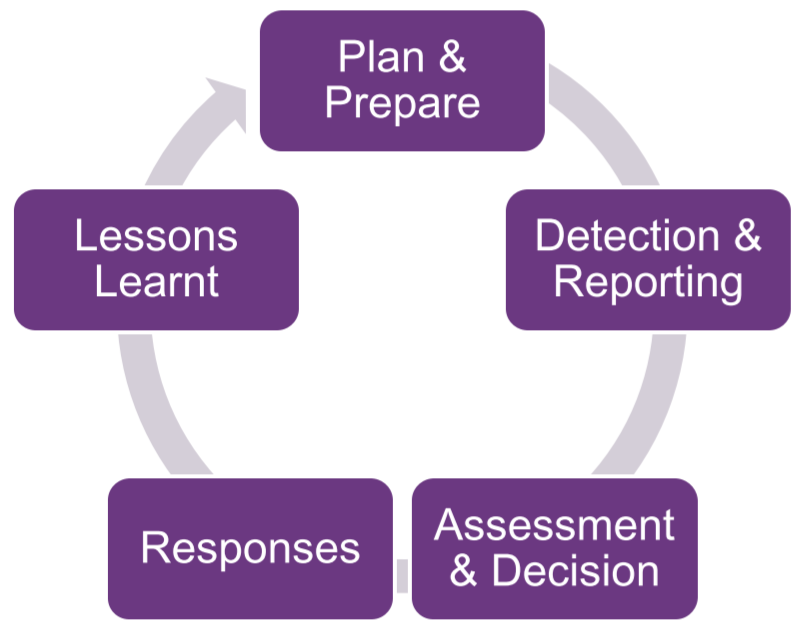
\includegraphics[width=.4\linewidth]{03-incresp_prozess/01-prozess}
    \vspace{-8pt}
\end{center}

\subsubsection{Plan \& Prepare}
\begin{itemize}
    \item Organisatorischen Incident Management Rahmen schaffen
    \item CEO/ Geschäftsführer muss vollstes commitment für Cyber Security zeigen
    \item Incident Management Plan festlegen
    \item Incident Response Team (IRT) etablieren
    \item Klassifikation festlegen, Formulare erstellen
    \begin{itemize}
        \item Damit im Notfall nicht wichtige Angaben im Formular vergessen gehen (z.B. SN Festplatte)
    \end{itemize}
    \item Intern \& extern vernetzen, vor allem verantwortliche Entitäten für Informationssicherheitsereignisse, -vorfälle \& Schwachstellenmanagement
    \begin{itemize}
        \item Connection/ Beziehungen aufbauen um im Notfall Zeit zu sparen
    \end{itemize}
    \item Trainieren, schulen, simulieren und Bewusstsein steigern (Red Teaming etc.)
    \item Fähigkeiten / Maturität überwachen
\end{itemize}

\paragraph{Ukraine Konflikt aus IR Sicht}
\begin{itemize}
    \item Heute die Projekte starten (jetzt ist Unterstützung GL sehr hoch)
    \item Geoblocking einschalten (auf FW)
    \item Logs beobachten/ Monitoring
    \item Low hanging fruits
    \item Awareness Kampagne
    \item Notfallkontakte überprüfen
    \item Tabletop Übungen
\end{itemize}

\begin{itemize}
    \item Genauer Ablauf sollte eine Organisation selber entwickeln (Incident Management Plan)
    \item Diverse Quellen können ein Ereignis feststellen und/oder melden (SIEM, FW, SOAR, EDR, etc.)
    \item \textbf{Wichtig}:
    \begin{itemize}
        \item Meldewege sind definiert
        \item Meldewege sind allen relevanten Parteien bekannt (Notfallnummernblatt)
        \item Empfänger der Meldung wissen, was damit zu tun ist
        \item Bei Meldequelle bedanken, Resultat/Folge der Meldung teilen $\rightarrow$ Meldungen motivieren!
    \end{itemize}
    \item IT-Sicherheitssysteme (technische Quellen)
    \begin{itemize}
        \item Proaktive Detektion vs. Reaktive Detektion
        \item Protokolle, SIEM, Schwachstellen-Scanner
        \item Deception Technologie, z. B. Honeypots, Honeytokens, Honey Accounts etc.
        \begin{itemize}
            \item Testen, ob Unternehmen Informationen weiterverkauft
            \item \textit{Honeypod} wird eine Einrichtung bezeichnet, die einen Angreifer oder Feind vom eigentlichen Ziel ablenken soll oder in einen Bereich hineinziehen soll, der ihn sonst nicht interessiert hätte (z.B. in Form eines Scheinziels).
        \end{itemize}
        \item Email Traps (Spamtrap), Sandbox
    \end{itemize}
    \item Wenn technische Quellen vorhanden sind und genutzt werden: Merkt jemand die Meldung?
    \begin{itemize}
        \item Automatisierung, unübersehbarer Alarm, SIEM (Aspekte der Cyber Defense)
    \end{itemize}
    \item Organisation
    \begin{itemize}
        \item Interne Partner: IT-Betrieb, Netzwerkbetrieb, IT Support
        \item externe Partner
        \begin{itemize}
            \item ISP, MSP (Managed Service Provider), IT-Dienstleister, Security-Partner, etc.
            \begin{itemize}
                \item Mit Dienstleistern Kommunikationspflicht festlegen
            \end{itemize}
            \item Cloud Dienstleister (SaaS, IaaS, PaaS, …) $\rightarrow$ Schattendienstleister
            \begin{itemize}
                \item Security-Kontakt einrichten
            \end{itemize}
            \item IT-Security-Partner, nationales CSIRT / NCSC
            \item Offene und geschlossene Gemeinschaften zum Informationsaustausch
        \end{itemize}
        \item Kommunikation im Vorfeld definieren!
        \item Medien
        \begin{itemize}
            \item Kann das Incident Response Team damit umgehen?
            \item Nein! Wenn Medien involviert sind:
            \begin{itemize}
                \item Public Relations, Marketing, Presseabteilung, … involvieren
                \item Geschäftsleitung sollte im Normalfall informiert werden
            \end{itemize}
        \end{itemize}
    \end{itemize}
    \item Mitarbeiter
    \begin{itemize}
        \item Wissen diese wo sie sich melden dürfen?
        \item Sind sie motiviert sich zu melden?
    \end{itemize}
    \item Externe Individuen
    \begin{itemize}
        \item White/Gray/Black Hats, Sicherheitsforscher, Bug Bounty usw.
        \item Have I Been Pwned, "Darknet Monitoring" / "Cyber Threat Intelligence"
    \end{itemize}
    \item Weiss der Empfänger/die Empfängerin, was mit einer Meldung zu tun ist?
\end{itemize}

\paragraph{Reporting}
\begin{itemize}
    \item \textbf{Ziel}: Wer, was, wo und wann für die weitere Verarbeitung festhalten.
    \begin{itemize}
        \item Wer hat es entdeckt? Wie erreichen wir diese Person?
        \item Was wurde wann beobachtet? Wo wurde es beobachtet?
        \item Wann wurde was bereits gemacht?
    \end{itemize}
    \item Je nach Organisation, Quelle und Auftrag diverse Formate denkbar:
    \begin{itemize}
        \item Mündlich am Telefon oder in Person
        \item Schriftliches oder digitales, vordefiniertes Formular
    \end{itemize}
\end{itemize}

\subsubsection{Assessment \& Decision}
\begin{itemize}
    \item \textbf{Ziel}: Feststellen, ob das Ereignis ein Vorfall ist
    \item Informationen zum Ereignis sammeln
    \item Entscheidung basierend auf Informationen:
    \begin{itemize}
        \item Kann es ein Vorfall sein? $\rightarrow$ Eskalation zum IRT (Incident Response Team)
        \item Ist es ein Vorfall? $\rightarrow$ IRT startet Response-Phase
        \item Ist es falschpositive Meldung? $\rightarrow$ Falschpositivenrate im Lessons Learnt senken
    \end{itemize}
    \item Wichtig: Spätestens ab hier detailliertes Protokollieren
    \begin{itemize}
        \item Was wurde wann, wo und von wem festgestellt?
        \item Welche Folgen hatte es?
    \end{itemize}
\end{itemize}

\subsubsection{Responses}
\begin{itemize}
    \item \textbf{Ziel}: Vorfall bewältigen/lösen
    \item Die Einschätzung (Klassifikation, Schweregrad etc.) fortlaufend neu bewerten
    \item Alle beteiligten Personen führen detailliertes Protokoll
    \item Beweise sammeln und sichern für eine mögliche spätere Untersuchung
\end{itemize}

\subsubsection{Lessons Learnt}
\label{incresp:prozess:iso:ll}
Lessons Learnt geht oft vergessen, ist aber sehr wichtig dass nicht wiederholt die gleichen Fehler gemacht werden.

\begin{itemize}
    \item Aus dem geschehenen lernen, analog einer Retrospektive oder einem Post Mortem
    \begin{itemize}
        \item Welche Schutzmassnahmen anpassen/verbessern?
        \item Wie können wir das Incident Management verbessern?
        \item Müssen wir unser Risikomanagement anpassen/ergänzen?
    \end{itemize}
    \item \textbf{Wird sehr gerne übersprungen / ignoriert}
    \item Absolut essenziell zur Steigerung der IT-Sicherheit und Reaktion auf Ereignisse/Vorfälle
\end{itemize}

\newpage

\subsection{SANS Incident Response Prozess}
\begin{center}
    \vspace{-8pt}
    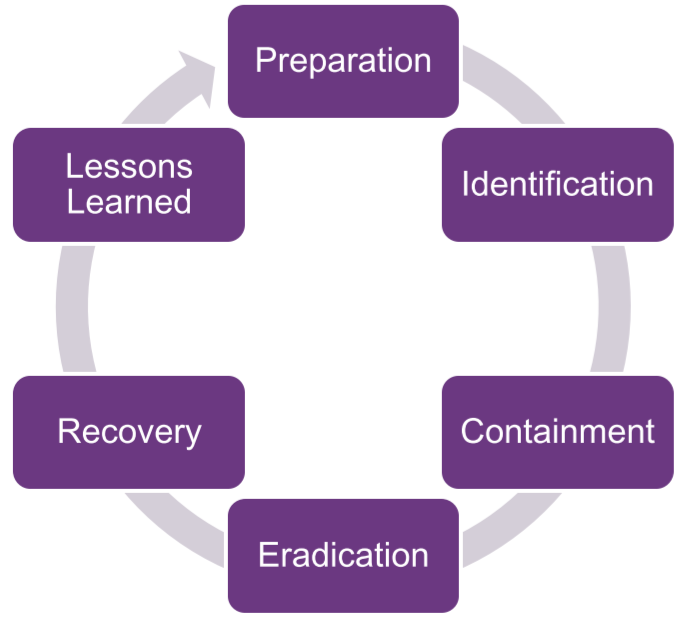
\includegraphics[width=.4\linewidth]{03-incresp_prozess/02-sans_prozess}
    \vspace{-8pt}
\end{center}

\subsubsection{Preparation}
\begin{itemize}
    \item Richtlinien, Prinzipien, Regeln etc. festlegen
    \item Prozess und Vorgehen für Vorfallbewältigung definieren
    \item Kommunikationsplan: intern, extern, Partner etc.
    \item Computer Incident Response Team (CIRT) definieren
    \item Notwendige Werkzeuge bereitstellen
    \item Trainieren
    \item \textbf{Ziel}: Technische und organisatorische Rahmenbedingungen vorbereiten/pflegen
\end{itemize}

\subsubsection{Identification}
\begin{itemize}
    \item Beginnt mit der Meldung eines möglichen Ereignisses
    \item Entscheiden, ob ein Ereignis vorliegt
    \item Prüfen, ob es ein Vorfall ist
    \item Spätestens in dieser Phase muss alles dokumentiert werden: Wer, was, wo, weshalb und wie
\end{itemize}

\subsubsection{Containment}
\begin{itemize}
    \item \textbf{Ziel}: Schaden mindern und weiteren verhindern
    \begin{enumerate}
        \item Kurzfristiges Containment: so früh wie möglich Schaden eingrenzen
        \item System Back-Up: Bevor Systeme zurückgesetzt werden diese forensisch sichern
        \item Langzeit Containment: Temporäre Massnahmen, bis Eradication abgeschlossen ist
    \end{enumerate}
\end{itemize}

\paragraph{Beispiel Containment}
\begin{itemize}
    \item Domain sperren
    \begin{itemize}
        \item Soll \lstinline|p.estonine.com| oder \lstinline|estonine.com| gesperrt werden?
    \end{itemize}
    \item IP-Adresse vom DNS Resource Record A (IPv4) und AAAA (IPv6) sperren
    \item In DNS Logs nach Domain suchen
    \begin{itemize}
        \item Domain ist ein Indicator of Compromise (IOC)!
    \end{itemize}
    \item In Firewall, Forward Proxy etc. Logs nach IP-Adresse suchen
    \begin{itemize}
        \item IP-Adresse ist ein IOC!
    \end{itemize}
    \item \textit{Scheduled Task} ist ein starker \textit{Indicator of Compromise (IOC)}
    \begin{itemize}
        \item Wird von Schadsoftware erstellt \& Name ist oft fest in Schadsoftware einprogrammiert
        \item Können mit PowerShell, WMI etc. nach Scheduled Tasks mit diesem Namen auf allen Windows-Systemen suchen
    \end{itemize}
\end{itemize}

\subsubsection{Eradication}
\begin{itemize}
    \item Schädliches und unerwünschtes entfernen
    \item Betroffene Systeme wiederherstellen ($\neq$ Backup wiederherstellen, zumindest nicht immer)
    \item System wieder in sauberen Zustand bringen (Malware entfernen, etc.)
\end{itemize}

\subsubsection{Recovery}
\begin{itemize}
    \item Betroffene Systeme wieder in den Betrieb bringen
    \item Vorsicht! Sollte nicht erneut zum Vorfall führen
    \begin{itemize}
        \item System überprüfen \& überwachen
    \end{itemize}
    \item Typische Herausforderung: Wann ist ein System \textit{sauber}?
\end{itemize}

\subsubsection{Lessons Learned}
Siehe \ref{incresp:prozess:iso:ll}

\subsection{NIST Incident Response LifeCycle}

NIST Standard mehr technisch, ISO Standard mehr fürs Management

\begin{center}
    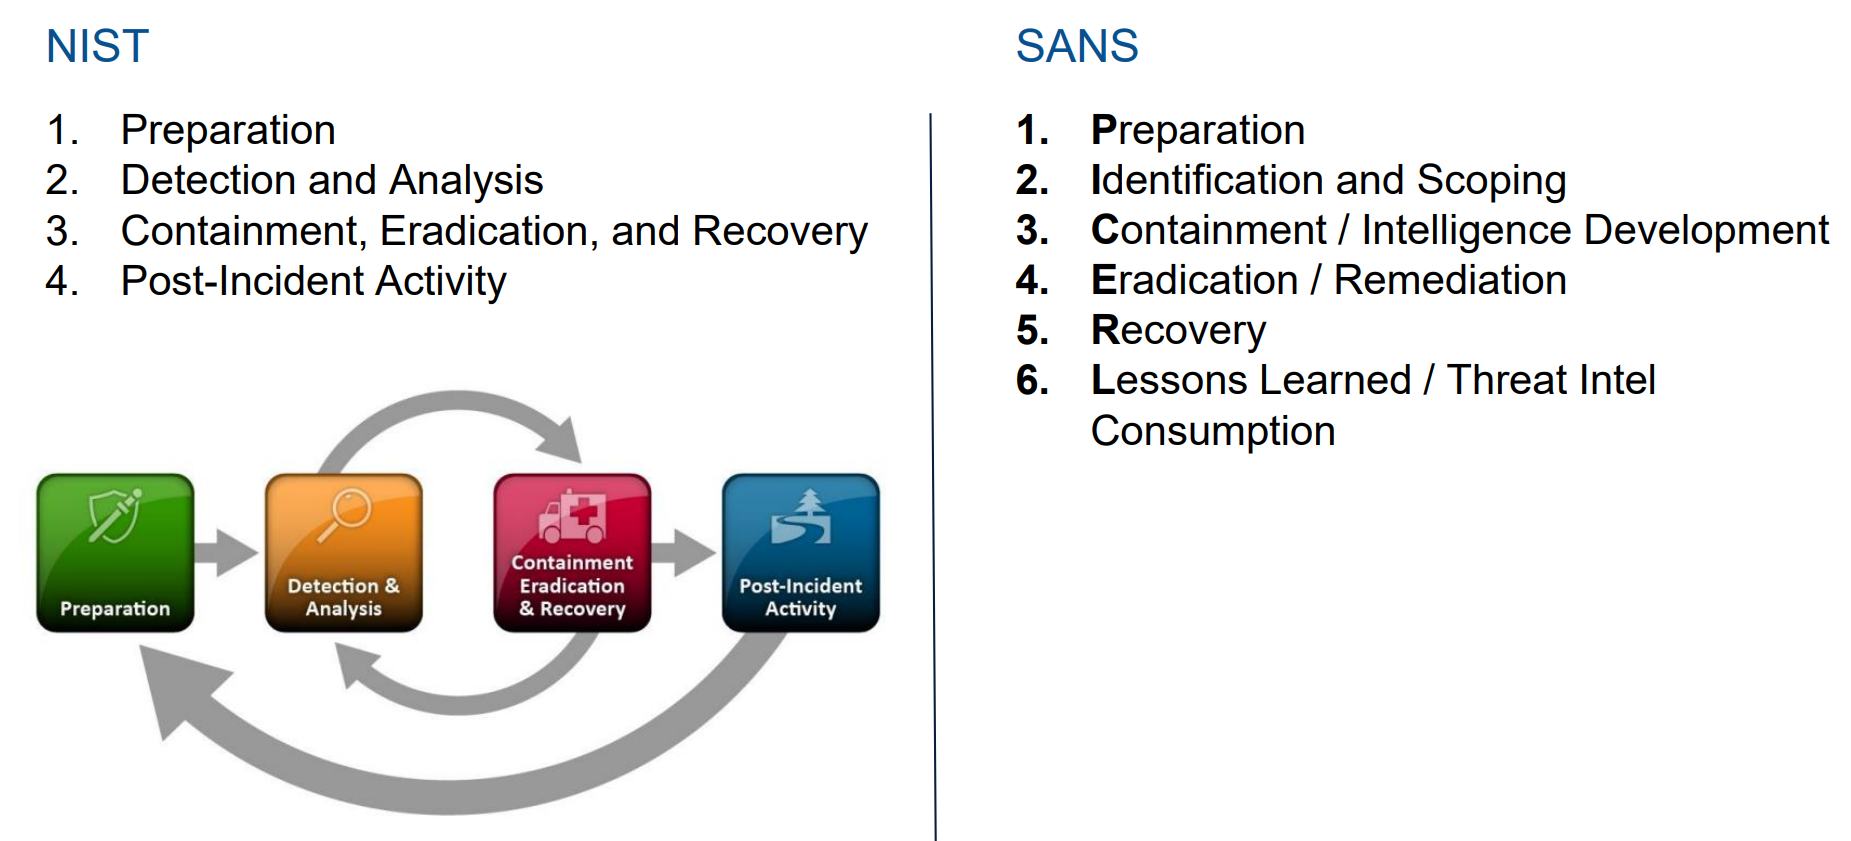
\includegraphics[width=1.0\linewidth]{03-incresp_prozess/04-nist_sans}
\end{center}

% TODO: Lernziele:
% Fragen zu den verschiedenen Phasen
% Etwa Wissen, was in welcher Phase gemacht werden sollte
% Was ist Containment, etc. (am besten mit Beispiel)
% Big-Picture Verständnis

% TODO: siehe Übung W02 + Quiz 2